\documentclass{jarticle}
\usepackage[dvipdfmx]{graphicx}
\usepackage{here}
\usepackage{listings,jlisting}


\lstset{
  basicstyle={\ttfamily},
  identifierstyle={\small},
  commentstyle={\smallitshape},
  keywordstyle={\small\bfseries},
  ndkeywordstyle={\small},
  stringstyle={\small\ttfamily},
  frame={tb},
  breaklines=true,
  columns=[l]{fullflexible},
  numbers=left,
  xrightmargin=0zw,
  xleftmargin=3zw,
  numberstyle={\scriptsize},
  stepnumber=1,
  numbersep=1zw,
  lineskip=-0.5ex
}

\title{{システム実験}\\実験12回レポート}
\author{6119019056 山口力也}
\date{2019/07/12日提出}

\begin{document}
\maketitle
\section{レポート7.2.1}
課題7.2.1で作成した装置について以下を報告せよ.
\begin{itemize}
\item プログラム(ArduinoとProcessing)
\item 実行結果のスクリーンショット
\item 物体の位置を正しく表示できたか?できなかった場合,その理由は何か?どんな改善が考えられるか?について考察せよ
\end{itemize}

以下ソースコード\ref{code:kadai7-2-1-a},ソースコード\ref{code:kadai7-2-1-p}にそれぞれ作成したプログラムのソースコードを示す.

\begin{lstlisting}[caption = 課題7.2.1(Arduino),label=code:kadai7-2-1-a][H]
#include <Servo.h>
#include <MsTimer2.h>

Servo servo; //Servo クラスのインスタンス servo を生成
const int trig = 7; //Trig ピンに接続する Arduino のピン番号
const int echo = 8; //Echo ピンに接続する Arduino のピン番号
const int servoPin = 11; //サーボモータの信号線に接続する Arduino のピン番号
unsigned long interval; //Echo のパルス幅(μs)
int distance; //距離(cm)
int angle; //回す角度
float wait; //待機時間
boolean clockwise = false; //時計回りかどうか

void setup() {
  Serial.begin(9600); //シリアル通信を 9600bps で初期化
  pinMode(trig, OUTPUT); //trig を出力ポートに設定
  pinMode(echo, INPUT); //echo を入力ポートに設定
  servo.attach(servoPin); //制御の対象を servoPin に割り当て
  angle = 0;
  wait = 80;
  //15秒で180度回転したいので
  //1度回転ごとに15 / 180秒待てば良い
  MsTimer2::set(wait,anglechange);
  MsTimer2::start(); //タイマ割り込みスタート

  // 
}
void anglechange() {
  servo.write(angle); //角度をサーボモータに出力
  if (clockwise)  angle --; //時計回りなら角度を小さくしていく
  else {
    angle ++; //半時計回りなら角度を大きくしていく
  }
  if (angle == 180) clockwise = true; //角度が180に到達したら時計回りに変更
  if (angle == 0) clockwise = false; //角度が0に到達したら半時計回りにする
}

void loop() {
  digitalWrite(trig, HIGH); //10μs のパルスを超音波センサの Trig ピンに出力
  delayMicroseconds(10);
  digitalWrite(trig, LOW);
  interval = pulseIn(echo, HIGH, 3452); //Echo 信号が HIGH である時間(μs)を計測
  //0.61*25 + 331.5 = 346.75
  //346.75 * x * 100 / 2 = 60
  //x = 3452
  distance = 340 * interval / 10000 / 2; //距離(cm)に変換
  
  if (distance > 60 ) { //距離が60cmを超えたら60とする
    distance = 60;
  } 
  Serial.write('H'); //ハンドシェイク用の記号
  Serial.write(distance); //距離を送信,60までなので1byteでok
  Serial.write(angle); //角度を送信,180までなので1byteでok
  delay(60);
   //Trig を再度 HIGH にするまでに 60ms 以上の間隔をあける(HC-SR04 の仕様)
   //この処理をしない場合、動作が不安定になる
}
\end{lstlisting}

\begin{lstlisting}[caption = 課題7.2.1(Processing),label=code:kadai7-2-1-p][H]
import processing.serial.*;

Serial port;
int distance; //距離(cm)
int angle; //角度(°)
int x; //対象のx座標
int y; //対象のy座標
float d_bef; //対象との距離(前回)
float d_now; //対象との距離(今)
void setup() {
  frameRate(60); //draw()を1秒間に60回呼び出す
  size(800,400); //600*200pxのウィンドウを作成
  background(255,255,255); //背景を白で描画
  port = new Serial(this, "/dev/ttyACM0",9600); //Serialクラスのインスタンスを生成
  d_bef = 0; //初期化
  d_now = 0; //初期化
}

void draw() {
  translate(400,400); //座標軸を(400,400)に移動
  
  strokeWeight(5); //線の太さを5に
  stroke(0,0,0); //線の色を黒に
  noFill(); //塗りつぶさない
  arc(0,0,800,800,-PI,PI); //(0,0)中心,直径800の半円を描画
  arc(0,0,400,400,-PI,PI); //(0,0)中心,直径400の半円を描画
  line(0,0,0,-height);
  strokeWeight(1);
  stroke(0,0,255);
  line(0,0,400 * cos(radians(angle)),-400 * sin(radians(angle)));
  stroke(255,0,0);
  d_now = map(distance,0,60,0,400); //距離を0~60から0~400に変える
  println(d_now);
  //if( d_now > 90 ) {
    if ( d_bef != d_now){
      ellipse(d_now*cos(radians(angle)),-d_now *sin(radians(angle)),8,8);
    }
  //}
  d_bef = d_now; //現在の値を過去の値として格納
  if ( angle == 180 || angle == 0 ) {
    background(255,255,255); //180度か0度になったら画面を初期化
  }
}

//シリアルポートにデータが到着するたびに呼び出される関数

void serialEvent(Serial p) {
  if ( p.available() >= 3){
    if (p.read() == 'H' ) {
      distance = p.read();
      angle = p.read();
      p.clear();
    }
  }
}
\end{lstlisting}

また,以下図\ref{fig:kadai7-2-1}に実行結果のスクリーンショットを示す.

\begin{figure}[H]
\begin{center}
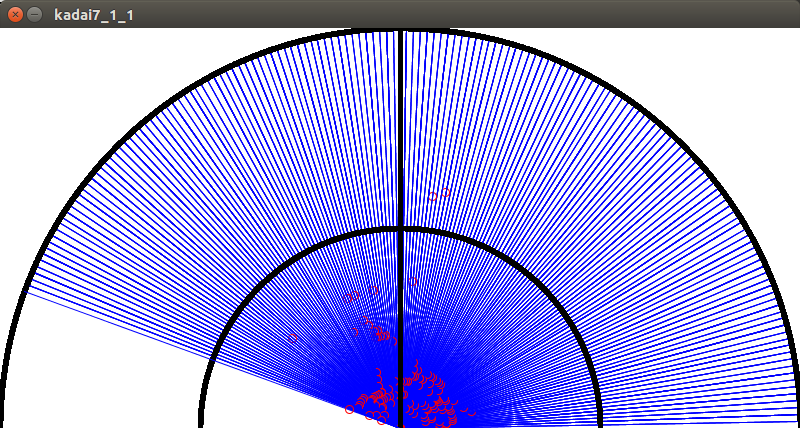
\includegraphics[width=7.0cm]{images/kadai7-2-1-yoi.png}
\caption{課題7.2.1の実行結果}
\label{fig:kadai7-2-1}
\end{center}
\end{figure}

比較的近い距離でノイズが現れて,物体の位置を正しく表示できなかった.これはエアコンの音や周りの音など,高周波の音が入ると超音波センサと干渉した結果ノイズとして表れたと考えられる.\\
改善方法としては2つあると考えられる.比較的近い距離でノイズが表れているためある一定の距離以下をプロットしないようにする方法が1つ.もう一つはローパスフィルタのようなものを通して高周波ノイズを除去することで他の環境音などと干渉した結果をカットしてしまう方法である.

\section{レポート7.2.2}
課題7.2.2で作成した装置について以下を報告せよ.
\begin{itemize}
\item プログラム(ArduinoとProcessing)
\item 実行結果のスクリーンショット
\item どのようなアルゴリズムでノイズを除去したか詳細に解説せよ.
\item 除去できなかったノイズがある場合,なぜ除去できなかったか考察せよ.
\end{itemize}


以下ソースコード\ref{code:kadai7-2-2-a},ソースコード\ref{code:kadai7-2-2-p}にそれぞれ作成したプログラムのソースコードを示す.

\begin{lstlisting}[caption = 課題7.2.2(Arduino),label=code:kadai7-2-2-a][H]
#include <Servo.h>
#include <MsTimer2.h>

Servo servo; //Servo クラスのインスタンス servo を生成
const int trig = 7; //Trig ピンに接続する Arduino のピン番号
const int echo = 8; //Echo ピンに接続する Arduino のピン番号
const int servoPin = 11; //サーボモータの信号線に接続する Arduino のピン番号
unsigned long interval; //Echo のパルス幅(μs)
int distance; //距離(cm)
int angle; //回す角度
float wait; //待機時間
boolean clockwise = false; //時計回りかどうか

void setup() {
  Serial.begin(9600); //シリアル通信を 9600bps で初期化
  pinMode(trig, OUTPUT); //trig を出力ポートに設定
  pinMode(echo, INPUT); //echo を入力ポートに設定
  servo.attach(servoPin); //制御の対象を servoPin に割り当て
  angle = 0;
  wait = 80;
  //15秒で180度回転したいので
  //1度回転ごとに15 / 180秒待てば良い
  MsTimer2::set(wait,anglechange);
  MsTimer2::start(); //タイマ割り込みスタート

  // 
}
void anglechange() {
  servo.write(angle); //角度をサーボモータに出力
  if (clockwise)  angle --; //時計回りなら角度を小さくしていく
  else {
    angle ++; //半時計回りなら角度を大きくしていく
  }
  if (angle == 180) clockwise = true; //角度が180に到達したら時計回りに変更
  if (angle == 0) clockwise = false; //角度が0に到達したら半時計回りにする
}

void loop() {
  digitalWrite(trig, HIGH); //10μs のパルスを超音波センサの Trig ピンに出力
  delayMicroseconds(10);
  digitalWrite(trig, LOW);
  interval = pulseIn(echo, HIGH, 3452); //Echo 信号が HIGH である時間(μs)を計測
  //0.61*25 + 331.5 = 346.75
  //346.75 * x * 100 / 2 = 60
  //x = 3452
  distance = 340 * interval / 10000 / 2; //距離(cm)に変換
  
  if (distance > 60 ) { //距離が60cmを超えたら60とする
    distance = 60;
  } 
  Serial.write('H'); //ハンドシェイク用の記号
  Serial.write(distance); //距離を送信,60までなので1byteでok
  Serial.write(angle); //角度を送信,180までなので1byteでok
  delay(60);
   //Trig を再度 HIGH にするまでに 60ms 以上の間隔をあける(HC-SR04 の仕様)
   //この処理をしない場合、動作が不安定になる
}
\end{lstlisting}

コードとしては\ref{code:kadai7-2-1-a}と同じものになる.

\begin{lstlisting}[caption = 課題7.2.2(Processing),label=code:kadai7-2-2-p][H]
import processing.serial.*;

Serial port;
int distance; //距離(cm)
int angle; //角度(°)
int x; //対象のx座標
int y; //対象のy座標
float d_bef_bef; //対象との距離(前々回)
float d_bef; //対象との距離(前回)
float d_now; //対象との距離(今)
void setup() {
  frameRate(60); //draw()を1秒間に60回呼び出す
  size(800,400); //600*200pxのウィンドウを作成
  background(255,255,255); //背景を白で描画
  port = new Serial(this, "/dev/ttyACM0",9600); //Serialクラスのインスタンスを生成
  d_bef = 0; //初期化
  d_now = 0; //初期化
}

void draw() {
  translate(400,400); //座標軸を(400,400)に移動
  
  strokeWeight(5); //線の太さを5に
  stroke(0,0,0); //線の色を黒に
  noFill(); //塗りつぶさない
  arc(0,0,800,800,-PI,PI); //(0,0)中心,直径800の半円を描画
  arc(0,0,400,400,-PI,PI); //(0,0)中心,直径400の半円を描画
  line(0,0,0,-height); //90度の線を描画
  strokeWeight(1); //線の太さを1に
  stroke(0,0,255); //線の色を青に
  //レーダーの線を描画
  line(0,0,400 * cos(radians(angle)),-400 * sin(radians(angle)));
  stroke(255,0,0); //線の色を赤に
  d_now = map(distance,0,60,0,400); //距離を0~60から0~400に変える
  println(d_now); //確認用
  if( d_now > 90 ) { //もし範囲が90以上なら
    if ( d_bef_bef == d_bef && d_bef == d_now){ //過去2回と現在の値を比較してすべて同じだったら
      //対象物として円を描画
      ellipse(d_now*cos(radians(angle)),-d_now *sin(radians(angle)),8,8);
    }
  }
  d_bef_bef = d_bef; //前回の値を前々回の値として格納
  d_bef = d_now; //現在の値を過去の値として格納
  if ( angle == 180 || angle == 0 ) {
    background(255,255,255); //180度か0度になったら画面を初期化
  }
}
//シリアルポートにデータが到着するたびに呼び出される関数
void serialEvent(Serial p) {
  if ( p.available() >= 3){ //送られてきたものが3つ以上なら
    if (p.read() == 'H' ) { //ハンドシェイク用の記号'H'が送られてきたら
      distance = p.read(); //距離を取得
      angle = p.read(); //角度を取得
      p.clear();
    }
  }
}
\end{lstlisting}

また,以下図\ref{fig:kadai7-2-2}に実行結果のスクリーンショットを示す.

\begin{figure}[H]
\begin{center}
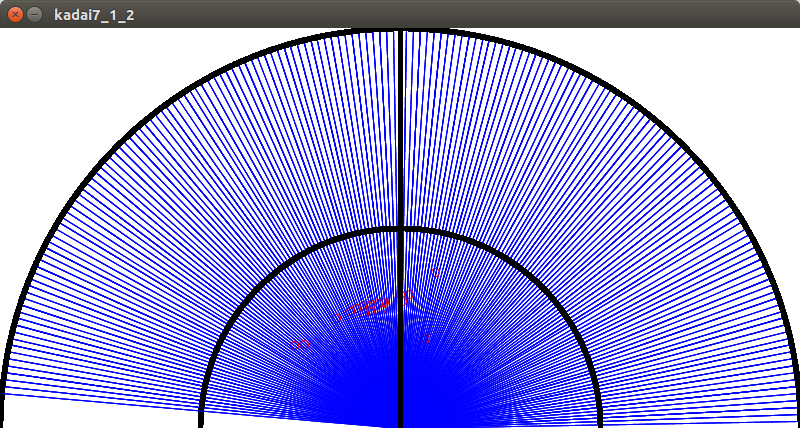
\includegraphics[width=7.0cm]{images/kadai7-2-2-yoi.png}
\caption{課題7.2.2の実行結果}
\label{fig:kadai7-2-2}
\end{center}
\end{figure}

\ref{fig:kadai7-2-1}で,比較的近い距離にノイズがあったことからある一定の距離より近い距離で対象を誤観測した場合はプロットしないようにした.実際の対象物はある程度の距離をもたせるようにした.しかしながらそれだけではまだ不完全だったため,前回と前々回の値を比較して全く同じ値であった場合プロットしないようにした.対象との距離が一定であった場合うまくプロットされない問題は残ったがノイズ自体は比較的除去できた.
除去できなかったノイズのようなものはないが,先程述べたとおり除去しすぎて実際に取りたいプロット(対象物の)が得られていないため改善する必要があると考えられる.
\section{発展課題レポート7.2.3}
発展課題7.2.3で作成した装置について以下を報告せよ.
\begin{itemize}
\item プログラム(ArduinoとProcessing)
\item 実行結果のスクリーンショット
\item どのようなアルゴリズムでノイズを除去したか詳細に解説せよ.
\item 正確にカウントできなかった場合,なぜカウントできなかったかを考察せよ.
\end{itemize}


以下ソースコード\ref{code:hatten7-2-3-a},ソースコード\ref{code:hatten7-2-3-p}にそれぞれ作成したプログラムのソースコードを示す.

\begin{lstlisting}[caption = 発展課題7.2.3(Arduino),label=code:hatten7-2-3-a][H]
#include <Servo.h>
#include <MsTimer2.h>

Servo servo; //Servo クラスのインスタンス servo を生成
const int trig = 7; //Trig ピンに接続する Arduino のピン番号
const int echo = 8; //Echo ピンに接続する Arduino のピン番号
const int servoPin = 11; //サーボモータの信号線に接続する Arduino のピン番号
unsigned long interval; //Echo のパルス幅(μs)
int distance; //距離(cm)
int angle; //回す角度
float wait; //待機時間
boolean clockwise = false; //時計回りかどうか

void setup() {
  Serial.begin(9600); //シリアル通信を 9600bps で初期化
  pinMode(trig, OUTPUT); //trig を出力ポートに設定
  pinMode(echo, INPUT); //echo を入力ポートに設定
  servo.attach(servoPin); //制御の対象を servoPin に割り当て
  angle = 0;
  wait = 80;
  //15秒で180度回転したいので
  //1度回転ごとに15 / 180秒待てば良い
  MsTimer2::set(wait,anglechange);
  MsTimer2::start(); //タイマ割り込みスタート

  // 
}
void anglechange() {
  servo.write(angle); //角度をサーボモータに出力
  if (clockwise)  angle --; //時計回りなら角度を小さくしていく
  else {
    angle ++; //半時計回りなら角度を大きくしていく
  }
  if (angle == 180) clockwise = true; //角度が180に到達したら時計回りに変更
  if (angle == 0) clockwise = false; //角度が0に到達したら半時計回りにする
}

void loop() {
  digitalWrite(trig, HIGH); //10μs のパルスを超音波センサの Trig ピンに出力
  delayMicroseconds(10);
  digitalWrite(trig, LOW);
  interval = pulseIn(echo, HIGH, 3452); //Echo 信号が HIGH である時間(μs)を計測
  //0.61*25 + 331.5 = 346.75
  //346.75 * x * 100 / 2 = 60
  //x = 3452
  distance = 340 * interval / 10000 / 2; //距離(cm)に変換
  
  if (distance > 60 ) { //距離が60cmを超えたら60とする
    distance = 60;
  } 
  Serial.write('H'); //ハンドシェイク用の記号
  Serial.write(distance); //距離を送信,60までなので1byteでok
  Serial.write(angle); //角度を送信,180までなので1byteでok
  delay(60);
   //Trig を再度 HIGH にするまでに 60ms 以上の間隔をあける(HC-SR04 の仕様)
   //この処理をしない場合、動作が不安定になる
}
\end{lstlisting}
コードとしては\ref{code:kadai7-2-1-a}と同じものになる.

\begin{lstlisting}[caption = 発展課題7.2.3(Processing),label=code:hatten7-2-3-p][H]
import processing.serial.*;

Serial port;
int distance; //距離(cm)
int angle; //角度(°)
int x; //対象のx座標
int y; //対象のy座標
float d_bef_bef; //対象との距離(前々回)
float d_bef; //対象との距離(前回)
float d_now; //対象との距離(今)
int count; //対象の個数をカウント
float count_d_bef;
float count_d_now;

void setup() {
  frameRate(60); //draw()を1秒間に60回呼び出す
  size(800,400); //600*200pxのウィンドウを作成
  background(255,255,255); //背景を白で描画
  port = new Serial(this, "/dev/ttyACM0",9600); //Serialクラスのインスタンスを生成
  d_bef = 0; //初期化
  d_now = 0; //初期化
  count = 0;
}

void draw() {
  translate(400,400); //座標軸を(400,400)に移動
  
  strokeWeight(5); //線の太さを5に
  stroke(0,0,0); //線の色を黒に
  noFill(); //塗りつぶさない
  arc(0,0,800,800,-PI,PI); //(0,0)中心,直径800の半円を描画
  arc(0,0,400,400,-PI,PI); //(0,0)中心,直径400の半円を描画
  line(0,0,0,-height); //90度の線を描画
  strokeWeight(1); //線の太さを1に
  stroke(0,0,255); //線の色を青に
  //レーダーの線を描画
  line(0,0,400 * cos(radians(angle)),-400 * sin(radians(angle)));
  stroke(255,0,0); //線の色を赤に
  d_now = map(distance,0,60,0,400); //距離を0~60から0~400に変える
  println(d_now); //確認用

  if( d_now > 90 ) { //もし範囲が90以上なら
    if ( d_bef_bef == d_bef && d_bef == d_now){ //過去2回と現在の値を比較してすべて同じだったら
      //対象物として円を描画
      ellipse(d_now*cos(radians(angle)),-d_now *sin(radians(angle)),8,8);

     }
  }
    
  if (abs(d_now - d_bef) > 10 && abs(d_bef - d_bef_bef) > 10){
    count++;
  }
  d_bef_bef = d_bef; //前回の値を前々回の値として格納
  d_bef = d_now; //現在の値を過去の値として格納

   if ( angle == 180 || angle == 0 ) {
    background(255,255,255); //180度か0度になったら画面を初期化
	 fill(0);
	 textSize(40);
	 text(count,-350,-350);
    count = 0; //カウントを初期化
  }
}
//シリアルポートにデータが到着するたびに呼び出される関数
void serialEvent(Serial p) {
  if ( p.available() >= 3){ //送られてきたものが3つ以上なら
    if (p.read() == 'H' ) { //ハンドシェイク用の記号'H'が送られてきたら
      distance = p.read(); //距離を取得
      angle = p.read(); //角度を取得
      p.clear();
    }
  }
}
\end{lstlisting}

また,以下図\ref{fig:hatten7-2-3}に実行結果のスクリーンショットを示す.

\begin{figure}[H]
\begin{center}
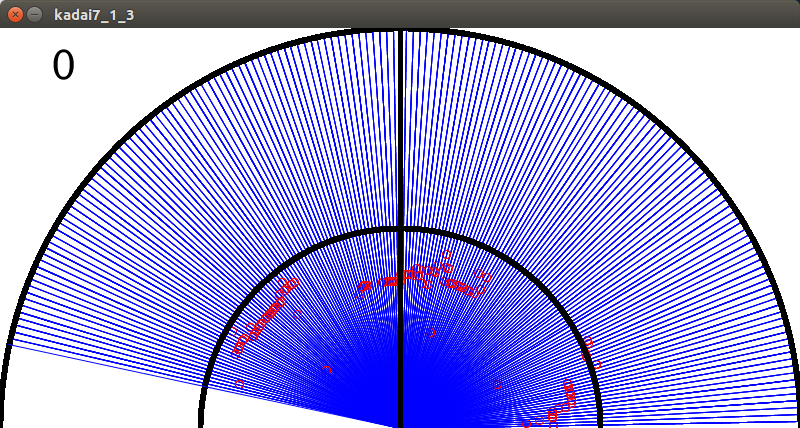
\includegraphics[width=7.0cm]{images/hatten7-2-3.png}
\caption{発展課題7.2.3の実行結果}
\label{fig:hatten7-2-3}
\end{center}
\end{figure}
アルゴリズムとしては距離が一定以上離れていた場合,過去2回の値と比較して現在の値と前回の値,前回の値と前々回の値を比較してそれぞれの距離(絶対値)が一定距離を超えていた場合カウントを増やすようにした.\\
また,正確にカウントできない場合が多くあったが,これは条件設定が難しいためだと考えられる.ある一定の距離というのが明確に示されておらず,実験的にこのくらいの距離だろうというのを確かめて設定したためその時々で曖昧な設定になりうまくカウントできなかったと考えられる.

\end{document}
